\emph{The Monitor Celestra} is a Nordic Style Live Action Roleplaying Game (LARP), organized for the first time in 2013. 
The game, situated
in the Battlestar Galactica\cite{larson_battlestar_1978} universe was a technology-heavy
immersive experience for the participants with ambitious goals to
transform the interior of a World War II era battleship into a
space ship and allow the participants to forge their own path into the future.

This full immersion was assisted by a host of different specific
techniques. For instance, all signage was replaced by new signs with the right
aesthetic to support the fiction, the ship had custom built control
panels that tied in with a space dynamics simulator, and the game
master team had access to triggering a large array of scripted, partially scripted or improvised events.

As a fundamental part of this, the ship was equipped with 15 pairs of
loudspeakers, each pair hooked up to a Raspberry Pi\cite{rpi} and
connected to a wired ethernet network. These loudspeakers played
localized sound effects as well as an ambient sound backdrop through
the entire game, drowning out the sounds of inner city Gothenburg and
supporting the game experience by confirming consequences of player
actions through mediated response.

\section{Background}
\label{sec:background}

LARP is a form of game where participants receive roles and then proceed to enact their roles within a framework of plots, story lines and clues. Traditionally LARPs have been focused on telling stories in a fantasy/medieval setting but has seen a wider spread of genres over years. LARP has developed into various design schools and style - mostly based on geographical distribution, thus one has Nordic LARP, American LARP and Russian LARP to name a few\cite{kp2011}. Each school of design has its own theories on what constitutes a good LARP and what goals one must strive to achieve with the game design, participation and outcome of the game. 

Stemming from table-top role playing games and improvisation theatre, LARP is played out by players in real time in the same general physical area. Players wear costumes and make props to better simulate their respective characters and there's usually a consensus of what is deemed \emph{in-game} vs. \emph{off-game}. In general, participants receive instructions beforehand regarding specific game rules, other characters, shared background information and similar. Organizers define social mechanics and hard game rules for resolving combat, conflicts or sex. 

\subsection{Nordic LARP}

\emph{The Monitor Celestra} belonged to the Nordic LARP school of design. This school could be argued to emphasize a few different points as being major when creating or participating in the experience: 

\begin{itemize}
\item The game should represent the world as faithfully and completely as possible, this is commonly referred to as a 360\degree{} game. Everything players see and/or experience represents itself within the game - a gun is a gun, a knife is a knife.
\item Participants should put emotional engagement and experience above achieving in-game goals. Powerful emotional impacts should take precedence when deciding how to move the game forward.
\item The players should control the outcome of the game. While parts of the game might be scripted, the main outcome of the game should be left in the players hand as far as possible.
\end{itemize}

Due to the nature of the Nordic school of design, games designed within that school tend to focus on moral choices and complex social interactions rather than traditional fantasy stories. There have been games depicting everything from danish hobos on the road in the LARP \emph{The White Road} \cite{pedersen2008}, students investigating possessed ladies in the LARP \emph{Prosopopeia} \cite{jonsson2006prosopopeia, montola2006prosopopeia} to 1950s families hiding from nuclear war in the LARP \emph{Ground Zero} and terminal cancer patients in the LARP \emph{Luminescence}, both described in \cite{nordiclarp}.

\subsection{LARP vs. Similar activities}

What separates LARP from other similar activities such as tabletop
roleplaying games, computer games or improvised theatre is still an
open question. Researchers \cite{montola2012,turku3,henriksen2004}
have pointed to a few main points; 

\begin{itemize}
\item Emotional engagements increased radically when players are physically engaged in the activity \cite{turku3}.
\item Moral choices and consequences from player actions have large impact when acted out by other physical players \cite{turku3}.
\item Players allow themselves more freedom when acting within a ludic circle,\musthavefootnote{\textit{ludic circle}: a shared space of playfulness, from \textit{ludic}: playful} thus allowing for a wider range of emotions, experiences and shared actions \cite{montola2012,stenros2012}.
\item Reflections on the complexity of social and/or humanistic behavior or models yield a high level of understanding \cite{henriksen2004}.
\end{itemize}

It has been humorously suggested that LARP may be seen as the extreme sport of interactive experiences due to the vast effort of both staging and participating in games, the powerful impact of properly designed and executed experiences and the cumulative effects of player actions and organizer design.

\subsection{Similar Events}

There has been other efforts to use technology to enhance LARP experiences, mainly within the Nordic school of LARP design. Historically, these experiments have been conducted by a small number of game designers and writers. Experiences where technology were used in a similar capacity as on \emph{The Monitor Celestra} includes: 

\begin{itemize}
\item \textbf{Prosopopeia: Bardo 1} A technology-enhanced LARP played in the autumn of 2005. Players used technology concealed in an old reel-recorder to communicated with dead spirits.
\item \textbf{Prosopopeia: Momentum} An ambitious continuation to the Prosopopeia project, \emph{Momentum} was played in the autumn of 2006 by 36 players for 30 days. Players used a wide variety of technology, including custom-built hardware to explore and wage battles against force on the other side of death. 
\item \textbf{Felsäkert Läge} A technology-enhanced LARP in the autumn of 2010 situated in a future, post-apocalyptic world, staged in an abandoned mining town in the north of Sweden. Technology was used to simulated surviving technology from before the catastrophe telling stories and providing quests, items and treasures for the players to find and use in their own game.
\end{itemize}

An overview of similar experiments (and others) can by found in \cite{nordiclarp}.

\subsection{Immersive Soundscapes}
Earlier efforts on immersive soundscapes include various implementations in Python, support in most holistic game engines and similar. However, the main difference between these implementations and the system built for \emph{The Monitor Celestra} is scale of spatiality. Often, these soundscapes are meant to be enjoyed by a single person in headphones or a handful of persons in a single or a few rooms. 

The difference in scale between these implementations and the one described in this paper makes comparisons hard to do. Most issues met by the usual implementations were either deemed irrelevant (such as super-focused spatial placement in the scene, a rough idea was more than enough for a battleship) or too specific (solutions for physical placing loudspeakers in a square room). 

\begin{figure}[H]
  \centering
  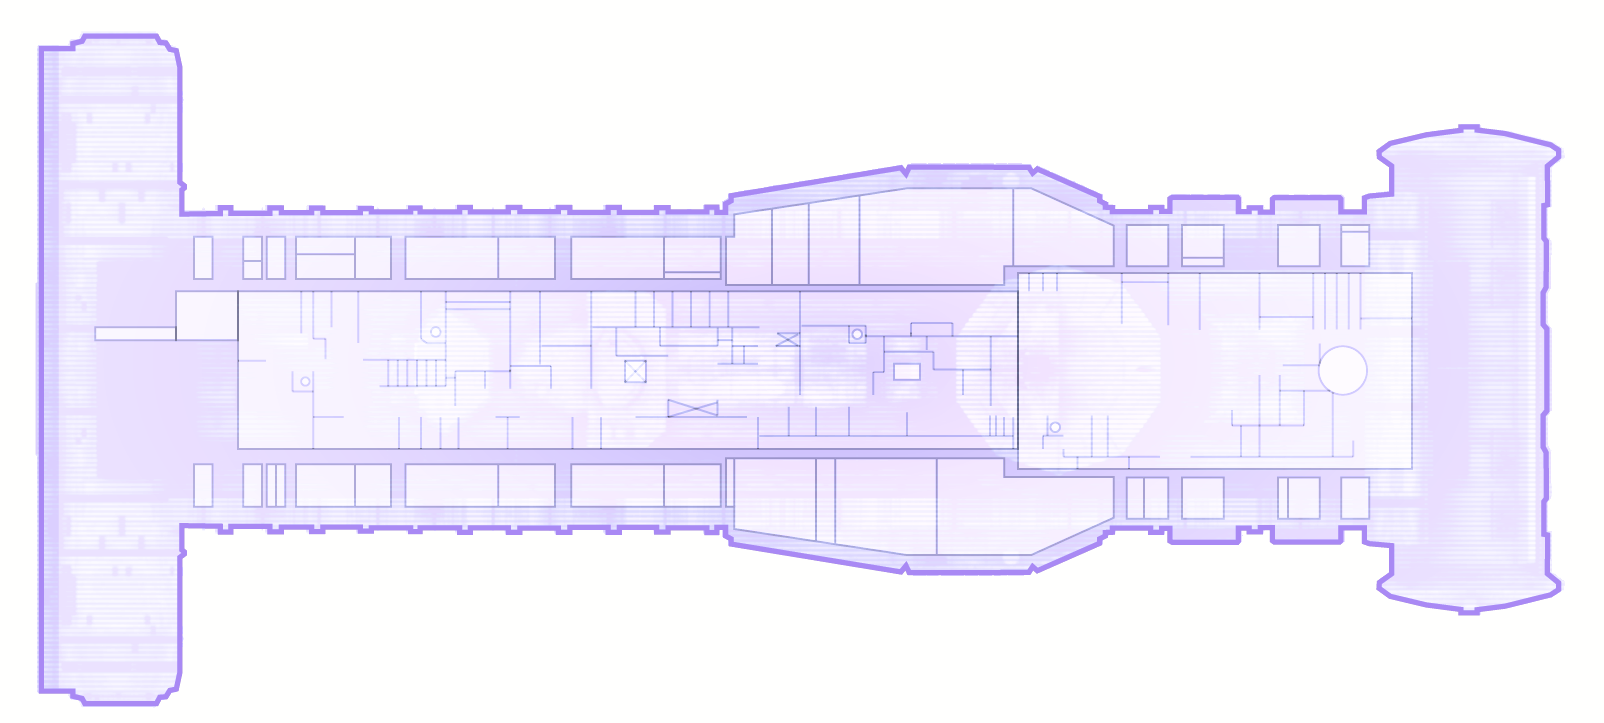
\includegraphics[width=0.6\textwidth]{img/ship}
  \caption{Floor plan of The Monitor Celestra}
  \label{fig:celestra}
\end{figure}

\subsection{Structure of The Monitor Celestra}
Every LARP differs in structure and design according to design goals, creators and aims with the project. The Monitor Celestra had three runs with 150 participants each, split over three weekends. The runs were separated from each other, and played out the same story with different participants (even though some participants bought tickets for all the runs). 

Every run was split into 4 game sessions at between 4--6 hours each, with breaks between for sleep and briefings. Food was distributed and eaten while in play. Even though the battleship Småland was equipped with bunks for its crew, fire regulations prohibit sleeping on board the ship. Hence, the participants slept at a nearby hostel between game days.

The game runs shared a common starting position in the story, and then took shape based on the participants actions - meaning that every game ended in a different way, ranging from a valiant effort to save the human race by nuclear suicide to setting course for deep space and forging a new path ahead.



%%% Local Variables: 
%%% mode: latex
%%% TeX-engine: default
%%% TeX-master: "tmr"
%%% End: 
